\subsection{Efficient convolution}

\begin{figure}[H]
    \centering
    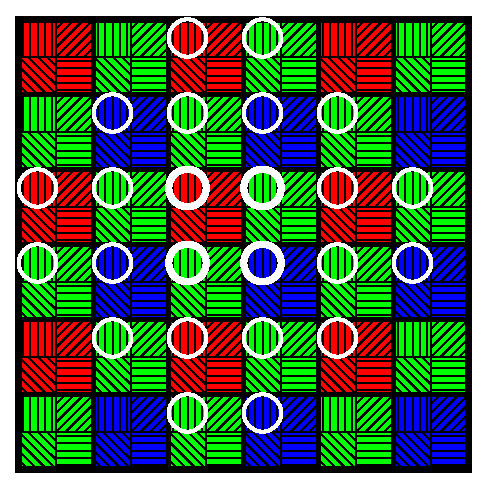
\includegraphics[width=.5\textwidth]{figures/polarized_image/normal_conv.pdf}
    \caption{Visualization of which pixels are used (white contour circle) to calculate the value of one Y value in the output image (filled white circle).}
    \label{fig:saperation}
\end{figure}


\begin{table}[H]
    \begin{minipage}[b]{.5\linewidth}
        \subcaptionbox{Separate debayering and color space conversion. Also shows where synchronization would be needed.}{
            \small
            \begin{tabular}{|l|c| c|}
                \hline
                \textbf{Operation}                         & \textbf{\# of \acrshort{fma}} \\
                \hline
                Green at red            (\ref{fig:mhc_gr}) & 9                             \\
                Green at blue           (\ref{fig:mhc_gb}) & 9                             \\
                Red at green 1 (\ref{fig:mhc_rgr})         & 11                            \\
                Red at green 2 (\ref{fig:mhc_rgb})         & 11                            \\
                Red at blue             (\ref{fig:mhc_rb}) & 9                             \\
                Blue at green 1 (\ref{fig:mhc_bgr})        & 11                            \\
                Blue at green 2 (\ref{fig:mhc_bgb})        & 11                            \\
                Blue at red             (\ref{fig:mhc_br}) & 9                             \\
                \textbf{\textit{Synchronize}}              &                               \\
                Convert to YCbCr                           & 36                            \\
                \textbf{\textit{Synchronize}}              &                               \\
                Binning Cb                                 & 4                             \\
                Binning Cr                                 & 4                             \\
                \hline
                \textbf{Total}                             & 124                           \\
                \hline
            \end{tabular}}
    \end{minipage}
    \begin{minipage}[b]{.5\linewidth}
        \subcaptionbox{Joined debayering and color space conversion.}{
            \small
            \begin{tabular}{|l|c|}
                \hline
                \textbf{Operation} & \textbf{\# of \acrshort{fma}} \\
                \hline
                Y at red           & 13                            \\
                Y at green 1       & 13                            \\
                Y at green 2       & 13                            \\
                Y at blue          & 13                            \\
                Cb                 & 24                            \\
                Cr                 & 24                            \\
                \hline
                \textbf{Total}     & 100                           \\
                \hline
            \end{tabular}}
    \end{minipage}
    \caption{Comparison of the number of \gls{fma} operations required to get the desired output. On the left }
\end{table}



\begin{listing}[H]
    \begin{minted}{cuda}
        __device__ __forceinline__ __half2 handle_u(__half2 **data, int col) {
            __half2 tmp = __float2half2_rn(5.000000000e-1f);
            tmp = __hfma2(__float2half2_rn(9.466415405e-5f), data[1][col + 1], tmp);
            tmp = __hfma2(__float2half2_rn(9.466415405e-5f), data[3][col - 1], tmp);
        \end{minted}
    \vspace{-26pt}
    \begin{minted}[linenos=false, autogobble=false]{cuda}
    ...
    \end{minted}
    \vspace{-26pt}
    \begin{minted}[firstnumber=24]{cuda}
        tmp = __hfma2(__float2half2_rn(-1.122532265e-5f), data[0][col], tmp);
        tmp = __hfma2_sat(__float2half2_rn(-1.122532265e-5f), data[2][col - 2], tmp);
        return __hfma2(__float2half2_rn(1023.0f), tmp, __float2half2_rn(0.0f));
    }
    \end{minted}
    \caption{Generated function}
    \label{listing:generated_function}
\end{listing}